\section{Ensemble Learning}
\label{sec:ensemble}
Um \textit{ensemble} é composto por um grupo de preditores (ou meta-classificadores), que nada mais são do que algoritmos clássicos de aprendizado de máquina. A técnica de combinar vários preditores é conhecida como \textit{Ensemble Learning} \cite{Geron:2017}. Existem vários métodos baseados nessa estratégia, os mais conhecidos na literatura são: \textit{bagging}, \textit{boosting} e \textit{stacking}.

\begin{figure}[h!]
    \centering
    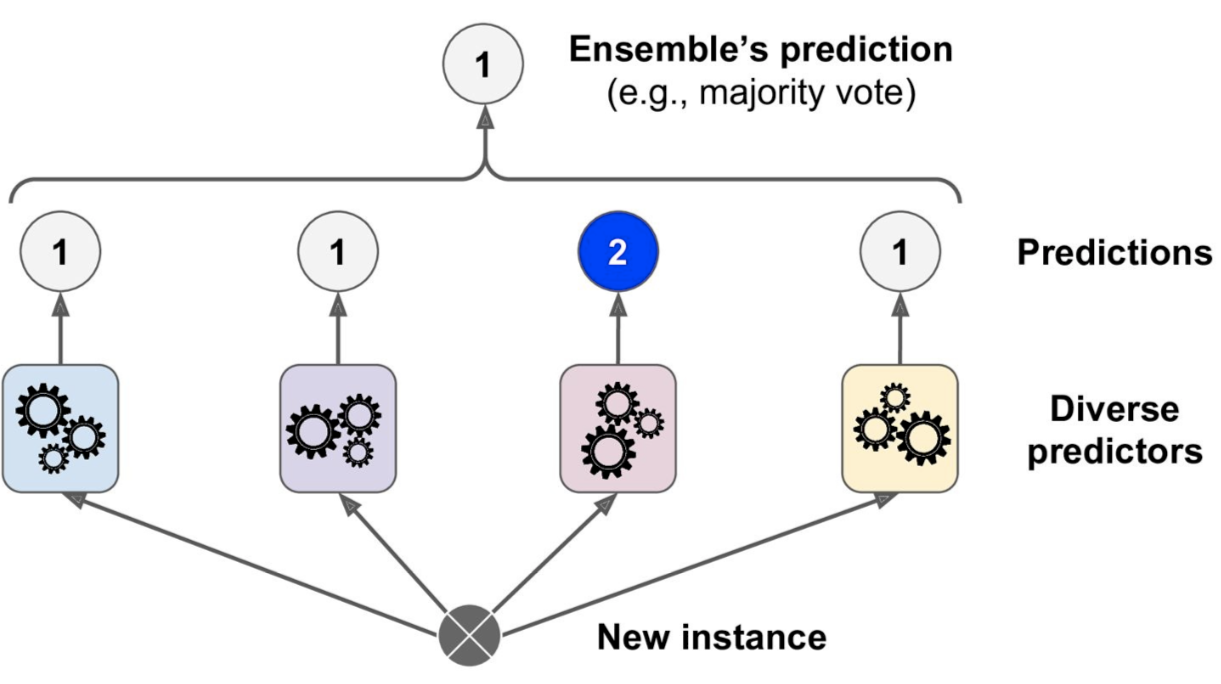
\includegraphics[scale=0.2]{Imagens/ensemble.png}
    \caption{Exemplo de um Ensemble Learning \cite{Geron:2017}}
    \label{fig:ensemble}
\end{figure}

Embora seja mais comum utilizar \textit{Ensemble Learning} para classificação, também é possível utilizar essa técnica para problemas de regressão.

Uma maneira muito simples de agregar os resultados de cada preditor, a fim de chegar em um classificar ainda mais robusto, é escolher a classe com a maior quantidade de votos. Essa estratégia é conhecida como \textit{Hard Voting Classifier}.

Contudo, é possível que haja classificadores bons e ruins, caso o número de preditores ruins supere o número de bons, é possível que o método \textit{ensemble} seja prejudicado e tenha um resultado inferior ao melhor preditor. Para contornar esse tipo de problema, uma estratégia possível é atribuir pesos diferentes para os preditores, essa estratégia é conhecida como \textit{Soft Voting Classifier}.


\subsection{Bagging e Pasting}
\hl{Inserir conteudo}